% This is "sig-alternate.tex" V2.1 April 2013
% This file should be compiled with V2.5 of "sig-alternate.cls" May 2012
%
% This example file demonstrates the use of the 'sig-alternate.cls'
% V2.5 LaTeX2e document class file. It is for those submitting
% articles to ACM Conference Proceedings WHO DO NOT WISH TO
% STRICTLY ADHERE TO THE SIGS (PUBS-BOARD-ENDORSED) STYLE.
% The 'sig-alternate.cls' file will produce a similar-looking,
% albeit, 'tighter' paper resulting in, invariably, fewer pages.
%
% ----------------------------------------------------------------------------------------------------------------
% This .tex file (and associated .cls V2.5) produces:
%       1) The Permission Statement
%       2) The Conference (location) Info information
%       3) The Copyright Line with ACM data
%       4) NO page numbers
%
% as against the acm_proc_article-sp.cls file which
% DOES NOT produce 1) thru' 3) above.
%
% Using 'sig-alternate.cls' you have control, however, from within
% the source .tex file, over both the CopyrightYear
% (defaulted to 200X) and the ACM Copyright Data
% (defaulted to X-XXXXX-XX-X/XX/XX).
% e.g.
% \CopyrightYear{2007} will cause 2007 to appear in the copyright line.
% \crdata{0-12345-67-8/90/12} will cause 0-12345-67-8/90/12 to appear in the copyright line.
%
% ---------------------------------------------------------------------------------------------------------------
% This .tex source is an example which *does* use
% the .bib file (from which the .bbl file % is produced).
% REMEMBER HOWEVER: After having produced the .bbl file,
% and prior to final submission, you *NEED* to 'insert'
% your .bbl file into your source .tex file so as to provide
% ONE 'self-contained' source file.
%
% ================= IF YOU HAVE QUESTIONS =======================
% Questions regarding the SIGS styles, SIGS policies and
% procedures, Conferences etc. should be sent to
% Adrienne Griscti (griscti@acm.org)
%
% Technical questions _only_ to
% Gerald Murray (murray@hq.acm.org)
% ===============================================================
%
% For tracking purposes - this is V2.0 - May 2012

\documentclass{sig-alternate-05-2015}
\usepackage{graphicx}
\usepackage{caption}
\usepackage{amsmath}
\DeclareMathOperator*{\argminA}{arg\,min}
\begin{document}

% Copyright
\setcopyright{acmcopyright}
%\setcopyright{acmlicensed}
%\setcopyright{rightsretained}
%\setcopyright{usgov}
%\setcopyright{usgovmixed}
%\setcopyright{cagov}
%\setcopyright{cagovmixed}


% DOI
\doi{}

% ISBN
\isbn{}

%Conference
\conferenceinfo{CGW '19}{June 27--28, 2019, Taoyuan City, Taiwan}

\acmPrice{}

%
% --- Author Metadata here ---
\conferenceinfo{CGW}{'19, June 27--28, 2019, Taoyuan City, Taiwan}
%\CopyrightYear{2007} % Allows default copyright year (20XX) to be over-ridden - IF NEED BE.
%\crdata{0-12345-67-8/90/01}  % Allows default copyright data (0-89791-88-6/97/05) to be over-ridden - IF NEED BE.
% --- End of Author Metadata ---

\title{Transition Motion Synthesis for Video-Based Text to ASL}
%\subtitle{[Extended Abstract]
%\titlenote{A full version of this paper is available as
%\textit{Author's Guide to Preparing ACM SIG Proceedings Using
%\LaTeX$2_\epsilon$\ and BibTeX} at
%\texttt{www.acm.org/eaddress.htm}}}
%
% You need the command \numberofauthors to handle the 'placement
% and alignment' of the authors beneath the title.
%
% For aesthetic reasons, we recommend 'three authors at a time'
% i.e. three 'name/affiliation blocks' be placed beneath the title.
%
% NOTE: You are NOT restricted in how many 'rows' of
% "name/affiliations" may appear. We just ask that you restrict
% the number of 'columns' to three.
%
% Because of the available 'opening page real-estate'
% we ask you to refrain from putting more than six authors
% (two rows with three columns) beneath the article title.
% More than six makes the first-page appear very cluttered indeed.
%
% Use the \alignauthor commands to handle the names
% and affiliations for an 'aesthetic maximum' of six authors.
% Add names, affiliations, addresses for
% the seventh etc. author(s) as the argument for the
% \additionalauthors command.
% These 'additional authors' will be output/set for you
% without further effort on your part as the last section in
% the body of your article BEFORE References or any Appendices.

\numberofauthors{2} %  in this sample file, there are a *total*
% of EIGHT authors. SIX appear on the 'first-page' (for formatting
% reasons) and the remaining two appear in the \additionalauthors section.
%
\author{
% You can go ahead and credit any number of authors here,
% e.g. one 'row of three' or two rows (consisting of one row of three
% and a second row of one, two or three).
%
% The command \alignauthor (no curly braces needed) should
% precede each author name, affiliation/snail-mail address and
% e-mail address. Additionally, tag each line of
% affiliation/address with \affaddr, and tag the
% e-mail address with \email.
%
% 1st. author
\alignauthor
Yulia\\
       \affaddr{National Taiwan University of Science and Technology}\\
       \affaddr{No.43, Keelung Rd., Sec.4}\\
       \affaddr{Taipei 10607, Taiwan}\\
       \email{m10609803@mail.ntust.edu.tw}
% 2nd. author
\alignauthor
Chuan-Kai Yang\\
       \affaddr{National Taiwan University of Science and Technology}\\
       \affaddr{No.43, Keelung Rd., Sec.4}\\
       \affaddr{Taipei 10607, Taiwan}\\
       \email{ckyang@cs.ntust.edu.tw}
}
% There's nothing stopping you putting the seventh, eighth, etc.
% author on the opening page (as the 'third row') but we ask,
% for aesthetic reasons that you place these 'additional authors'
% in the \additional authors block, viz.
%\additionalauthors{Additional authors: John Smith (The Th{\o}rv{\"a}ld Group,
%email: {\texttt{jsmith@affiliation.org}}) and Julius P.~Kumquat
%(The Kumquat Consortium, email: {\texttt{jpkumquat@consortium.net}}).}
%\date{30 July 1999}
% Just remember to make sure that the TOTAL number of authors
% is the number that will appear on the first page PLUS the
% number that will appear in the \additionalauthors section.

\maketitle
\begin{abstract}
This paper describes a novel approach to provide a text to ASL media, a Video-Based Text to ASL. The hearing impaired or we called as the Deaf are used to communicate using Sign Language. When they have to face the spoken language, they have difficulties to read the spoken words as fast as the hearing people. The availability of a public dataset named ASL Lexicon Dataset give the challenge to make the video-based interpreter for the Deaf. After the dataset has been pre-processed, they are fed to OpenPose library to extract the skeleton of the signers and save it as JSON files. The system require the user to input some glosses by text, then it will find the JSON files and the videos for the corresponding glosses. The whole sequence of original video is also fed into the system to be used as a transition pulls. Later, the corresponding frames of the glosses are inputted together with the transition pulls to construct the sequence transition frames. After getting the sequences, to enhance the smoothness of the motion, we also apply one cross-faded frame between every transition we chose. Since this algorithm is fully depends on the transition pulls, there are some limitation regarding to make a good transition. If the transition frames we need to make a logically and visually correct motion are not available, then the result will be not optimized. But as long as the frames we need are available, this system can generate a logically and visually correct transitions.
\end{abstract}


%
% The code below should be generated by the tool at
% http://dl.acm.org/ccs.cfm
% Please copy and paste the code instead of the example below. 
%
\begin{CCSXML}
	<ccs2012>
	<concept>
	<concept_id>10003120.10003121</concept_id>
	<concept_desc>Human-centered computing~Human computer interaction (HCI)</concept_desc>
	<concept_significance>500</concept_significance>
	</concept>
	<concept>
	<concept_id>10003120.10003121.10003128.10011753</concept_id>
	<concept_desc>Human-centered computing~Text input</concept_desc>
	<concept_significance>100</concept_significance>
	</concept>
	<concept>
	<concept_id>10010147.10010371.10010352.10010380</concept_id>
	<concept_desc>Computing methodologies~Motion processing</concept_desc>
	<concept_significance>500</concept_significance>
	</concept>
	<concept>
	<concept_id>10010147.10010371.10010382.10010383</concept_id>
	<concept_desc>Computing methodologies~Image processing</concept_desc>
	<concept_significance>500</concept_significance>
	</concept>
	<concept>
	<concept_id>10010147.10010371.10010387</concept_id>
	<concept_desc>Computing methodologies~Graphics systems and interfaces</concept_desc>
	<concept_significance>500</concept_significance>
	</concept>
	<concept>
	<concept_id>10010405.10010469.10010473</concept_id>
	<concept_desc>Applied computing~Language translation</concept_desc>
	<concept_significance>500</concept_significance>
	</concept>
	<concept>
	<concept_id>10002951.10003227</concept_id>
	<concept_desc>Information systems~Information systems applications</concept_desc>
	<concept_significance>300</concept_significance>
	</concept>
	<concept>
	<concept_id>10003752.10003790</concept_id>
	<concept_desc>Theory of computation~Logic</concept_desc>
	<concept_significance>100</concept_significance>
	</concept>
	<concept>
	<concept_id>10003752.10003809</concept_id>
	<concept_desc>Theory of computation~Design and analysis of algorithms</concept_desc>
	<concept_significance>100</concept_significance>
	</concept>
	</ccs2012>
\end{CCSXML}

\ccsdesc[500]{Human-centered computing~Human computer interaction (HCI)}
\ccsdesc[100]{Human-centered computing~Text input}
\ccsdesc[500]{Computing methodologies~Motion processing}
\ccsdesc[500]{Computing methodologies~Image processing}
\ccsdesc[500]{Computing methodologies~Graphics systems and interfaces}
\ccsdesc[500]{Applied computing~Language translation}
\ccsdesc[300]{Information systems~Information systems applications}
\ccsdesc[100]{Theory of computation~Logic}
\ccsdesc[100]{Theory of computation~Design and analysis of algorithms}

%
% End generated code
%

%
%  Use this command to print the description
%
\printccsdesc

% We no longer use \terms command
%\terms{Theory}

\keywords{Sign Language; ASL; OpenPose; Deaf talk; Transition Motion Synthesis}

\section{Introduction}
According to World Health Organization (WHO)~\cite{deafnessAndHearingLoss}, there are over 5\% or about 466 million of world's population have suffered of hearing disability. This number consists of 432 million adults and 34 million children. It is also predicted that by 2050, there will be over 900 million people or one in every ten people will have the hearing disability.

Sign Languages are the natural languages developed by the Deaf, the communities of people who mostly have profound hearing loss which indicates very little or no hearing, all over the world with their own grammar and lexicon. American Sign Language (ASL) is a natural language which dominates sign language of the Deaf in the US and most of Anglophone Canada. Not only North America, the dialects of ASL and ASL-based creoles are also used in many countries including much West Africa and parts of South East Asia. ASL have some phonemic components, including movement of the face and torso together with the hands.

It has been proved that the reading ability of the deaf high school students are equal to the hearing students which are seven years younger. The median reading skills of Deaf students between 8 and 18 years old are equal to the hearing students in their fourth grade. The lack of phonemic awareness does have a big impact to their reading fluency.

Regarding the importance of ASL for Deaf, Athitsos et al.~\cite{ASLLexiconVideoDataset} made the availability of ASL Lexicon Video Dataset, a public dataset containing video sequences of thousands of distinct ASL signs, along with the annotations of those sequences. The dataset is made with the objectives to develop a vision-based system that allows users, the hearing communities, to look up the meaning of an ASL sign and is proposed to be used for gesture and sign recognition. 

Based on the second previous paragraph and the availability of a video-based dataset, the idea to provide a video-based translation system from English to ASL for the Deaf has risen. The scope of this research focuses on how to provide transitions between videos instead of leave it blinks.

\section{Literature Review}
Sign languages are the natural languages developed by each Deaf community all over the world with their own grammar and lexicon, which means each community has their own grammar and lexicon~\cite{WendySandler:2006}. This means that sign languages are unique for each region, not universal and not mutually intelligible.

It has been proved that the reading ability of the deaf high school students are equal to the hearing students which are seven years younger. The median reading skills of Deaf students between 8 and 18 years old are equal to the hearing students in their fourth grade. The lack of phonemic awareness does have a big impact to their reading fluency. The Deafs are at a disadvantage compared to the hearing individuals because they cannot implicitly learn the relationship between letters and sounds without direct instruction and access to sound

Some systems to provides an interpreter media for the Deaf to understand the spoken language have already proposed for years. For example, ~\cite{DeafTalkUsing3DAnimatedSignLanguage},~\cite{ChineseLanguageAnimation},~\cite{tessa},~\cite{signlanguageanimationusingtvml},~\cite{3danimationframeworkforsignlanguage} who have made contributions for this field using 3D animation media. The input can be text or sounds that later be processed into keywords then the pre-stored 3D animations are played on the screen based on the input. Tools that commonly used by the works are MakeHuman to make the model or by getting some provided model resource, Blender to create the animation, or by using sensors used to capture every Sign Language gesture from a real human and translate it to avatar-based interpreter. In so far as we know from the previous works, every spoken language to ASL translator used avatar-based method to generate the interpreter since the 3D animation

American Sign Language (ASL) is a natural language which dominates sign language of Deaf communities in the United States and most of Anglophone Canada. Not only North America, the dialects of ASL and ASL-based creoles are also used in many countries, including much West Africa and parts of South East Asia. ASL have some phonemic components, including movement of the face and torso together with the hands.

The public ASL dataset provided by Athitsos et al.~\cite{ASLLexiconVideoDataset} was performed by native ASL signers. It has almost 3.000 signs contained in the Gallaudet Dictionary of American Sign Language. The video was captured at 30 frames per second with resolution 1600x1200 pixels per frame. It also covered several angle side of the signer. In other words, a video can contain several words and everytime the signer start or end their gesture movement, the gesture of putting hands on the thigh are shown which we called by resting part. This dataset was provided to be a dictionary to find the meaning of an ASL meaning and is hoped to promote research towards developing vision-based methods sign language recognition on a markerless images. 

OpenPose is a library made to detect 2D human body from 2D images and videos. Instead of detecting one person, this library can also detect multiple people in the same image or video in a real time manner. It uses a non-parametric representation named Part Affinity Fields to learn to connect the body parts with the individuals in the images or videos. OpenPose is also the first open-source realtime system to detect multi-person in 2D manner including the body, foot, hand and the facial keypoints. This library also provide a quick start mode using their own pretrained model. It also provides APIs for C++ and Python language.

Animating objects in a still pictures has also been done by Xu et al.~\cite{AnimatingAnimalMotionFromStill}. This research is about making a motion animation of animal from a still image. It assumes a still picture of moving animals contains a hint about their motion. So, the main idea of this work is to extract every individuals from the picture and make a motion path in the graph connecting motion snapshots to infer the order of the motion. The animating method uses morphing among the ordered snapshots so the animation will be looked smoother.

\section{Methodology}
This section mainly focuses on the real implementation of the proposed system. Firstly, it will talk more about the adoption and the behavior that is done to the ASL dataset. Then, we come up with the algorithm to make the transition.

\subsection{ASL Lexicon Video Dataset}
The most important part for doing Sign Language is the hand movement. Since for each gesture performed by the signer was recorded in a side view, two frontal views and a view zoomed in on the face, we choose the frontal view with the upper body is visible since we want to show the hand movement clearly for the viewer.

A video from ASL Lexicon Video Dataset contains a sequence of words performed by a signer. Although the signer is a native ASL user, the recording moment required the signer to follow a guide to perform word by word. After they perform a word, they have to look into the guide for several seconds to perform the next word. While paying attention to the guide, the cameras were still recording them. Therefore, we can see the signers put their hands on their thigh for many times in a sequence of video, and we call it as "resting pose".

In this research, the videos we choose only contain one same signer from several ASL signers to make a possible good continuity from word to word. Because each video sequence contains multiple signs, we also cut them manually into one word per video based on the annotation provided. The annotation itself has the gloss of  the gestures and the start and end time of them excluding the resting pose.

\subsection{OpenPose Library}
After we got the one word per video dataset, we use the help of OpenPose library~\cite{openpose1}~\cite{openpose2}~\cite{openpose3}~\cite{openpose4} to acknowledge the human body information of the signers. The library itself can well detect face, body and hands of individuals inside an image or a video. Body parts detected such as face, body, and hands has its own annotation. The face has 70 keypoints, body has 25 keypoints, and hands which are divided into left and right palm has 21 keypoints for each of them.

We use the pretrained model provided by this library to extract the skeleton of body and hands of the signers. The extracted frames is saved as JSON files regarding the number of video frames and stored in a same folder named the gloss of the gesture. Beside extracting the pose information from one word per video dataset, we also extract the pose for the whole original video dataset and make it as our transition pose pulls. 

\begin{figure}
	\centering
	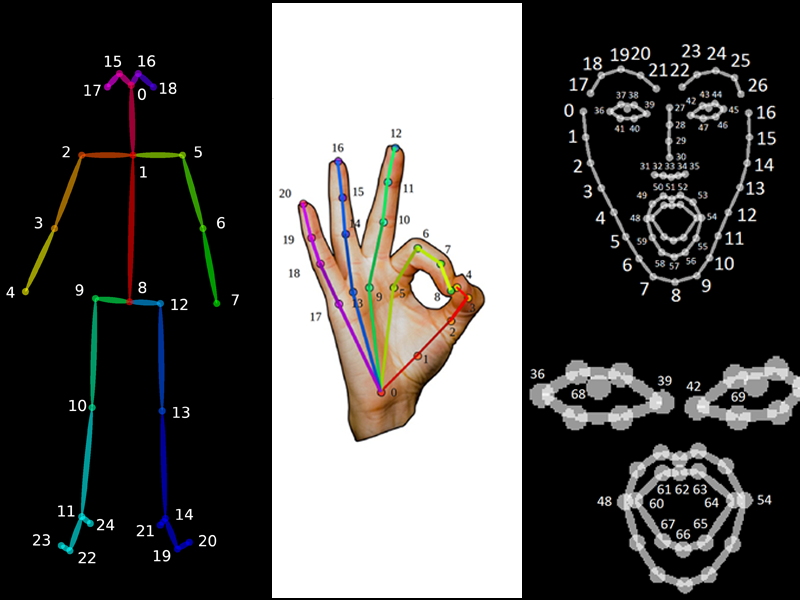
\includegraphics[width=\linewidth]{img/openpose.png}
	\caption{OpenPose Keypoints Output Format. Cited from GitHub source of~\cite{openpose1}~\cite{openpose2}~\cite{openpose3}~\cite{openpose4}.}
\end{figure}

\subsection{Constructing Transition Frames}
Combining glosses from the input can be quite complicated as the initial and the terminating positions of each gesture is not same. A great dislocation of the body part to perform the next gesture will be significantly exist and resulting blinks for every transition from one word to another word.

Regarding to the big difference of the starting and the ending gestures and the original video dataset recording which made the signer did resting pose from word to word, we can not perform a learning technique to generate the transition from word to word for our cut word videos because there is no frame can be used as the training set.

By using the similar concept of Xu et al.~\cite{AnimatingAnimalMotionFromStill} work, we came up with the idea to find the best frames which can be put together to make a transition from the whole sequence video instead of trying to generate it using Deep Learning. The assumption for this following algorithm to be succeed is the frames which have similarities with the corresponding input frames must exist.

\subsubsection{Keypoints Selection}
As what we described before, we try to adapt the help of OpenPose library to detect the signer. So simply put, our method does not conduct to use any other image processing methods. We got the help of mathematics to solve the next problem.

To reduce the complexity of the JSON format, we try to select some important keypoints instead of doing calculations using every stored keypoints. We tried to analyze the video and found for our research, we just need to take attention to the wrist, palm center and fingertips orientation of the signer that can be got from OpenPose body part with keypoint index 4 and 7 for the wrist, hand part with keypoint index 0 for the palm center and keypoint index 4,8,12,16, and 20 for the fingertips (see Fig. 1).

\subsubsection{Similarity Measurement}
Because we already had the location of the wrist, palm center and fingertips estimated location using the library, we try to operate the similarity measurement using L2 norm distance and cross product to find the orientation. The L2 norm distance is implemented to calculate the similarity between the wrist and palm center keypoints, and the cross product is implemented to the fingertips.

\begin{figure*}
	\centering
	\includegraphics[width=\textwidth]{img/process.png}
	\caption{Main Process of The Proposed System}
\end{figure*}

\begin{equation}d(p,q)=d(q,p)=\sqrt{(q_1-p_1)^2+(q_2-p_2)^2}\end{equation}

where \begin{math}p\end{math} and \begin{math}q\end{math} are the x and y of the keypoints location. We assume that the wrist and the palm center can be used for finding the similar frames because the wrist and the palms center are the most stable keypoints compared to fingers which have a big degree of freedoms resulting many possibilities to move around the space.

\begin{equation}c(p,q)=p_x q_y-p_y q_x\end{equation}

The above equation is a cross product implemented in the system which just has 2 dimension, x and y. Originally cross product is used to produce a vector that is perpendicular to the other two vectors, counting how much torque a force was applied to a rotating system, and how much the vector field is 'curling' up. Because it results a vector, usually the dimension of the vector given is more than two. Since we just have x and y location, so we assume the z is 0. We use cross product to get the rotation of the fingers based on the thumb tip position that is used as the center of mass. This rotation can give us a meaning of fingers orientation, whether the palm is facing the camera or the location of the fingers based on the thumb.In this case, \begin{math}p\end{math} equals to thumb tip keypoint, and \begin{math}q\end{math} is various from the index fingertip to the pinkie fingertip. 

\begin{equation}sim(F)=d(w\_L)+d(w\_R)+d(pc\_L)+d(pc\_R)+x\end{equation}

Where \begin{math}sim(F)\end{math} is the similarity measurement result for transition frame candidate F. w\_L and w\_R are wrist left and wrist right. pc\_L and pc\_R are palm center left and palm center right.

For every cross-product result, if the orientation of the corresponding fingers from the current transition frame candidate with the \begin{math}n\end{math}-last frames from the corresponding gloss is different, we added some values into the similarity result to make the value bigger, and let us declare it as \begin{math}x\end{math}. The less the similarity value, the opportunity to be a part of transition frames is bigger, and vice versa.

\subsubsection{Composing Transition Frames Sequence}
To compose the transition frames sequence, n-last frames from the previous input gloss and n-last frames from the next input gloss are selected to be used in similarity measurement section. Several frames from previous and next gloss are needed as we want to make sure that the result is not overly based only on the last and first frame of the previous and next gloss. The result should be similar with the corresponding gloss frames and is hoped to be able to connect the gesture from the previous to the next gloss. So, instead of measuring the distance from two frames (transition candidate frame and the input frame), we do the calculation for \begin{math}2n\end{math} times.

\begin{equation}
\begin{aligned}
sim(F)=\sum_{i=1}^{2n}d(w\_L)w_i+\sum_{i=1}^{2n}d(w\_R)w_i+\\
 \sum_{i=1}^{2n}d(pc\_L)w_i+\sum_{i=1}^{2n}d(pc\_R)w_i+x
\end{aligned}
\end{equation}

where \begin{math}i=1...n\end{math} is the \begin{math}n\end{math}last frames from previous gloss, and \begin{math}i=n+1...2n\end{math} is the \begin{math}n\end{math} first frame from the next gloss. \begin{math}w_i\end{math} is the weight for each corresponding input gloss frames.

The arrangement of the transition frames sequence is divided into two parts, left and right division. Since we have the weight parameter that will be bigger on the left and end with bigger weight on the right. Bigger weight means the resulting frame will be much more similar with the bigger weight frames rathe than the smaller one.

For each division, we feed the \begin{math}n\end{math}-last frames from the previous gloss and \begin{math}n\end{math}-last frames from the next gloss to the similarity measurement function. The returned frame will be the one most similar frame regarding to the calculation and weight variable for once the similarity function is called. The difference between the division is on which index the returned frame should be placed and which fed frames has bigger weights. 

\begin{figure}
	\centering
	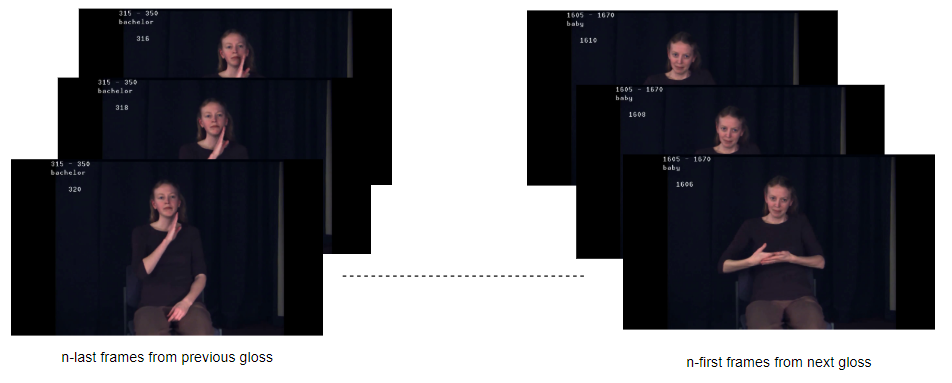
\includegraphics[width=\linewidth]{img/ncorrframes.png}
	\caption{n-Last Frames from Previous Gloss and n-First Frames from Next Gloss}
\end{figure}

The left division is run first, then will be continued by the right division. For the left division, the returned frame is always inserted at the very first (inserted on the first index of the list) of the transition frames sequence. The frames which are inserted to the similarity measurement in the next iteration is the n-last frames from the previous gloss and the \begin{math}n\end{math}-last temporary transition frames sequence. If the temporary transition frames has not met the \begin{math}n\end{math}-number, the first rest of \begin{math}n\end{math}-frames from the next gloss will be fed. Not forgetting to remove the returned frame from the transition pulls candidate to avoid receiving the same frame for the next iteration.

In the contrary with the right division, every time it received the one most similar frames from the function, the frame will be put in the very last (append the list) of the transition frames sequence for the right division itself. So, for the next iteration it also feeds the contrary behavior. It will fed the \begin{math}n\end{math}-first temporary transition frames sequence with the \begin{math}n\end{math}-first frames from the next gloss because we want the first most similar frame placed right next to the first frame of the next gloss and vice versa.

Therefore, the weight variable also have an important part to decide which frames to be returned. The left division are set to have bigger weight for the very last n frame of the previous gloss, then getting smaller for the next gloss because it has to emphasize the similarity of the transition frame candidate with the previous gloss. The right division also set on the contrary way too. it has a smaller weight for the corresponding previous gloss frames, and bigger value for the next gloss frames.

This method is run iteratively from the left division until it met the threshold which are bigger than the last returned transition frame similarity value, then is continued by the right division and also be stopped by the threshold.

\begin{figure}
	\centering
	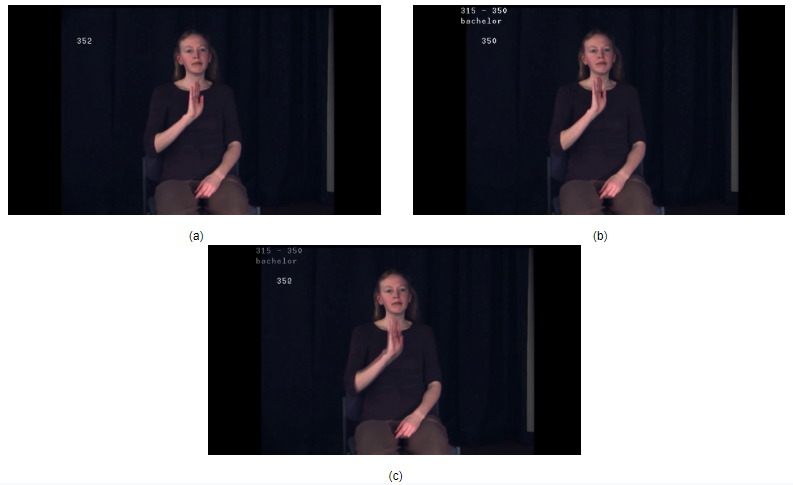
\includegraphics[width=\linewidth]{img/crossfading.png}
	\caption{Additional Crossfaded Frame. (a) The previous frame. (b) The next frame. (c) Crossfading result.}
\end{figure}

\subsubsection{Outliers Prevention}
In this work, the term outliers are given to frames which can not be put in between the input gloss as a part of the transition, but can be possibly inserted because it is assumed to be the most similar frame for the fed frames regarding to the distance calculation. To prevent the outlier, we also have to follow the trajectories of the corresponding frames.

\begin{equation}
\begin{aligned}
f^\ast = \argminA_{f \varepsilon F} Sim(f) ,
F=\{f|min_x<f_x<max_x  \land  \\
min_y<f_y<max_y\}
\end{aligned}
\end{equation}

where \begin{math}f^\ast\end{math} means the resulting transition frame, \begin{math}f\end{math} is a set of keypoints from the corresponding frame from the transition pulls \begin{math}F\end{math}, \begin{math}min_x\end{math} and \begin{math}max_x\end{math} are the minimum and the maximum \begin{math}x\end{math} location of the corresponding keypoints from the very last and very first frame of the previous and the next gloss, and so for \begin{math}min_y\end{math} and \begin{math}max_y\end{math}.

\subsubsection{Animation Smoothing}
Assume that we have arranged the transition frames in the correct order, sometimes the jitter for the motion still exist. To make it smoother, we also adopt the cross-fading technique which is used to insert one additional frames in between with pixels valued the average of the previous and the next frames. The main objectives of the cross-fading is making a fade out effect for the previous frame and fade in for the next frame. We are currently also trying to adopt image morphing to enhance the smoothness.

\section{Experimental Result}
After explaining the methods, in this section mentioned the parameters and variables we use. We also conducted a small user study for a temporary analysis of our current work.

\subsection{Parameters}
For our system, we choose to set n-frames to 3. So for every similarity measurement iteration, the function have to calculate the similarity between a transition frame candidate with 3 last frames from the previous gloss and 3 first frames from the next gloss.

Fingertip orientation variable also adjusted to the returned value of the distance regarding the width and height of the frame. In this case, we increase the similarity value by 40 for each different orientation of finger.

The left division part has increasing weights: 0.6, 0.8, and 1 for the last three frames from the previous gloss and decreasing weights 0.6, 0.4, 0.2 for the first three frames from the next gloss and vice versa for the right division.

The threshold is also set into a fix number by doing experiment and decreased as the iteration goes by. The more iteration we do, the more unexpected transition frames retrieved. The similarity value retrieved from one iteration to another also getting smaller because the previous and the next gloss is getting nearer since we already inserted some transition in-between. Therefore, to stop the iteration we also have to reduce the threshold to some number for each iteration and if the most similar frames similarity value is bigger than the threshold, the iteration will be stopped. 

\begin{figure}
	\centering
	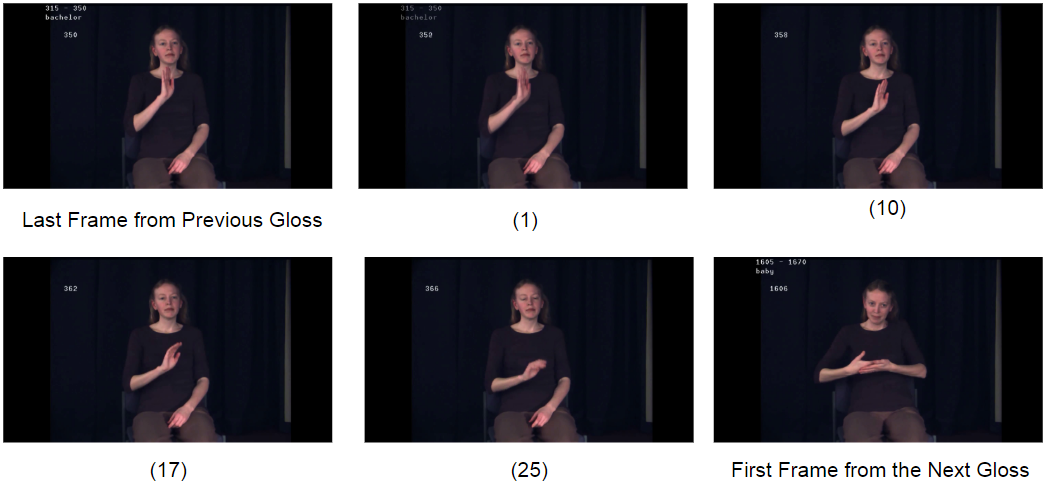
\includegraphics[width=\linewidth]{img/success.png}
	\caption{Success Case (I). There are 25 synthesized frames to connect two glosses.}
\end{figure}

Fig. 5 shows the first success case example from the experiment. As we can see in the caption below it, there are 25 frames be inputted in-between to make a possible transition of the hand gesture from the last frame from the previous gloss to the next frame to the previous gloss. Although as we can see for the transition between frame number 25 and the first frame from the next gloss still suffers a big movement, but the algorithm are succeed to try it best to find some previous transition frames with a logically and visually correct direction to continue to the next gloss gesture.

\begin{figure}
	\centering
	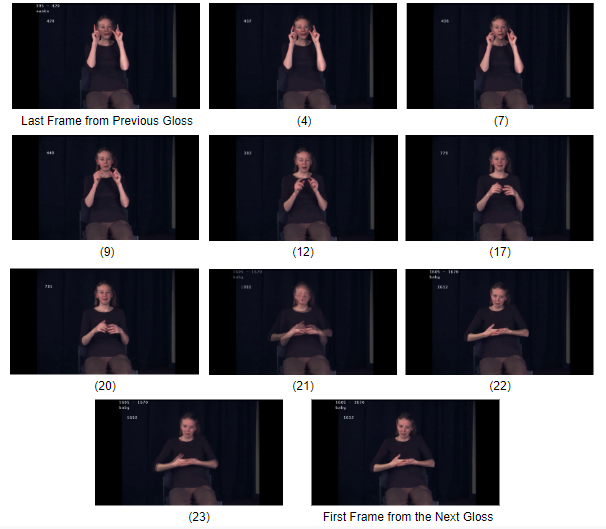
\includegraphics[width=\linewidth]{img/success1.png}
	\caption{Success Case (II). There are 23 synthesized frames to connect two glosses.}
\end{figure}

Fig. 6 shows the second success case example which produced 23 transition frames put in between the glosses. This second example shows a better result than the first one because the previous gloss on this fig. 6 performs a two-hand gesture and followed by a two-hand gesture for the next gloss. So, the transition we got seems have better continuance from frame to frame.

As we can see in Fig. 7, although it has more transitions in-between the last and first frame of the glosses, the transition is not logically and visually correct. For example the transition number 22 and 25, the signer performs a scratching body gesture which are irrelevant with the desired transition. It can be happened because of the threshold, the condition to stop the iteration is not suitable for this pair of words. The direction of the hands also cannot be mentioned as a correct path. Transition number 31 and the first frame from the next gloss have too much difference. This is happened because there is no possible similar frames of gesture that can be put in.

\begin{figure}
	\centering
	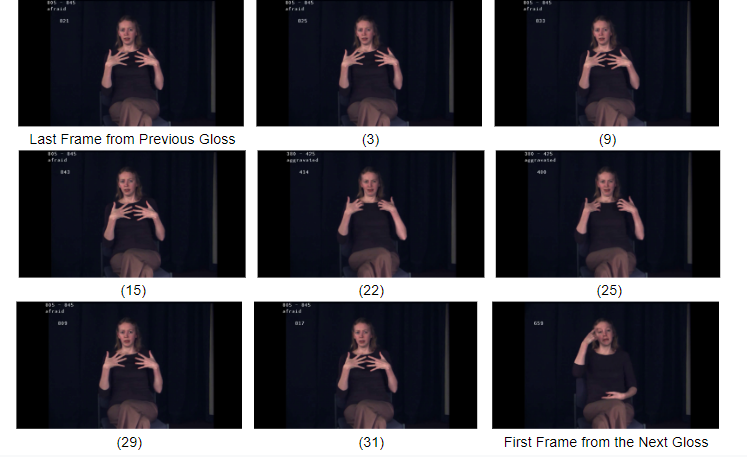
\includegraphics[width=\linewidth]{img/failure.png}
	\caption{Failure Case. There are 31 synthesized frames to connect two glosses.}
\end{figure}

We group the failure and success case by the final difference we can achieve. If the distance stays in a significant amount and cannot be decreased anymore, then we classify it as a failure. For the last two frames in Fig. 5 and Fig. 7 we can see the movement difference are relatively bigger than the previous frames. But, we classify Fig. 5 as a success case because although it cannot find any similar frame with the first frame for the next gloss, the difference of it with the last transition frame are smaller than in Fig. 7 and the direction or the optical flow from the previous transition frames can cover the transition movement well enough. 

\subsection{User Study}
There are five hearing people with no background of ASL knowledge who has tried to look into the result. Firstly, they were given a whole sequence of video contained the corresponding glosses. We asked them to pay more attention when the glosses we picked were shown.

Then we showed them the cut videos without our transitions for the corresponding gloss and ask them to also pay attention to the motion movement from a gloss to another gloss. Not forgetting to let them remembering the gesture.

Lastly, we also ask them to pay attention on our work. We gave the users time to understand the gesture and the transition we made.

From this user study, four people mentioned the video with transition inserted is better and prefer to watch it than the without transition one, and they feel the transition does not change the meaning of the main gestures. One person said the video with transition inserted is also better but has no big difference with the without transition one.

Later we want to target the real Sign Language users to join our experiment with a hope that our system can help them to get a better experience of generating a video from spoken language to ASL using video-based method which contained a real human interpreter.

\section{Conclusions}
This paper proposed a novel algorithm to produce a video-based text to ASL using a publicly stored dataset, ASL Lexicon Dataset. Since the words were performed separately in a sequence of video, we have to cut them based on the preserved annotation and store them as different individuals. Later, we use OpenPose, a library to detect people skeleton for each video and store them as JSON files. We also select some important keypoints to reduce the calculation complexity. 

The input for this proposed algorithm are some glosses which are available in the dataset, then the system finds the related video and JSON and processed them using the proposed method. The result shows that this algorithm has some limitation, such as the system will find a difficulties when a signer perform a one-hand gesture then followed by a two-hands gesture or vice versa. 

Because this algorithm fully depends on the frames availability within a transition pulls and there is no frame that can connect from one-hand gesture frame to two-hands gesture frame. The variable also takes a direct role to the results. Besides, if the glosses received has a small difference, or has the same number of hands to do the gesture, it can produce a logically and visually correct transition frames. 

An enhancement of the smoothness also appear by the help of cross-fading. This research is still an ongoing work and will be continued by implementing morphing. Besides, we also want to target the real Sign Language users community to help us doing the experiment to verify our results.

%
% The following two commands are all you need in the
% initial runs of your .tex file to
% produce the bibliography for the citations in your paper.
\bibliographystyle{abbrv}
\bibliography{sigproc}  % sigproc.bib is the name of the Bibliography in this case
% You must have a proper ".bib" file
%  and remember to run:
% latex bibtex latex latex
% to resolve all references
%
% ACM needs 'a single self-contained file'!
%
%APPENDICES are optional
%\balancecolumns



%\balancecolumns % GM June 2007
% That's all folks!
\end{document}
